\documentclass{article}

\usepackage{graphicx}
\usepackage{tikz}
\usepackage{tikzsymbols}
\usetikzlibrary{calc,patterns,shapes.geometric}
\pagestyle{empty}
\usepackage[margin=0pt]{geometry}
\geometry{papersize={14in,12in}}

\def\centerarc[#1](#2)(#3:#4:#5){\draw[#1] ($(#2)+({#5*cos(#3)},{#5*sin(#3)})$) arc (#3:#4:#5);}

\begin{document}
	\begin{figure}
		\centering
		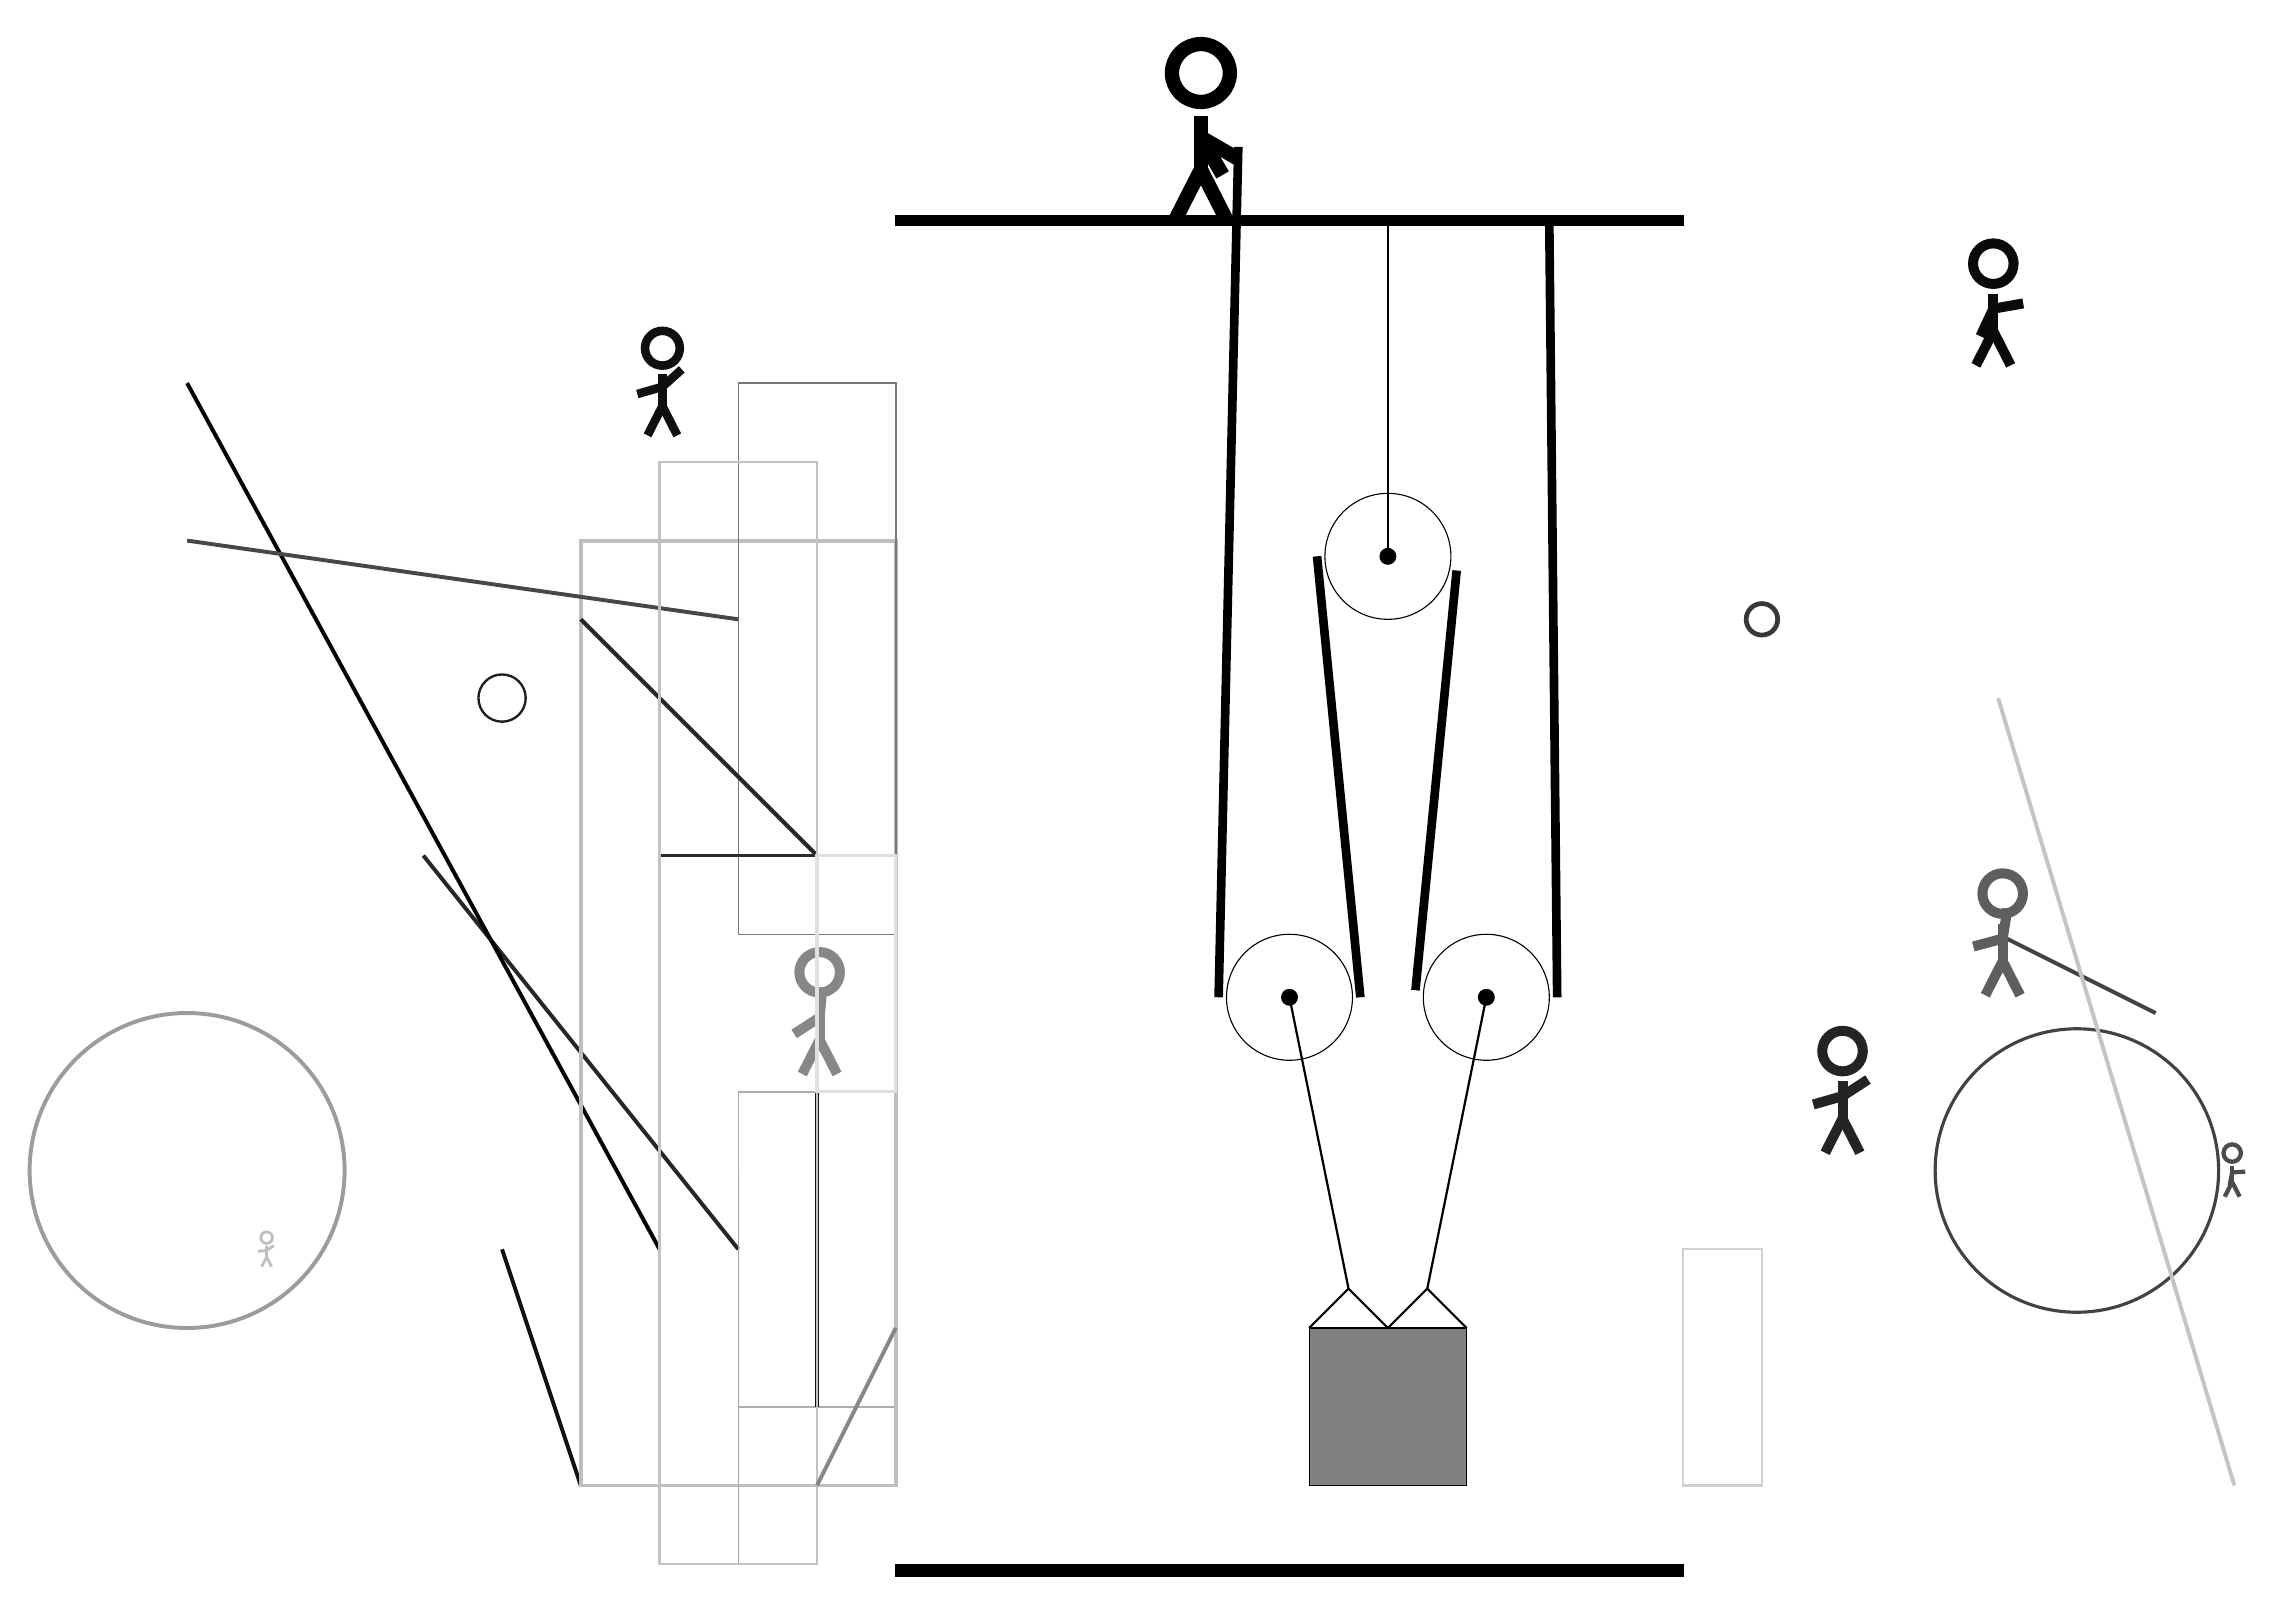
\begin{tikzpicture}
			%%%%% START %%%%%
			
			\draw[fill=black] (-4, 14) rectangle (6, 14.125);
			
			\draw (1, 4.2) circle (0.8);
			\draw[fill=black] (1, 4.2) circle (0.1);
			
			\draw (2.25, 9.8) circle (0.8);
			\draw[fill=black] (2.25, 9.8) circle (0.1);
			\draw[thick] (2.25, 9.8) -- (2.25, 14);
			
			\draw [line width=0.4mm, color=black!74](11, 2) circle (1.8);
			
			\draw[line width=0.5mm, color=black!85](-6, 1) -- (-10, 6);
			\draw[line width=0.2mm, color=black!32] (-6, -1) rectangle (-4, 3);
			\node[line width=0.2mm, color=black!94] at (-7, 12) {\Strichmaxerl[6][16][42]};
			\draw[line width=0.5mm, color=black!93](-8, -2) -- (-9, 1);
			\draw [line width=0.5mm, color=black!39](-13, 2) circle (2.0);
			\draw[line width=0.5mm, color=black!99](-7, 1) -- (-13, 12);
			\draw[line width=0.5mm, color=black!74](10, 5) -- (12, 4);
			\draw [line width=0.4mm, color=black!59](-5, 5) circle (0.0);
			\node[line width=0.5mm, color=black!25] at (-12, 1) {\Strichmaxerl[2][5][34]};
			\draw[line width=0.3mm, color=black!18] (7, 1) rectangle (6, -2);
			\node[line width=0.2mm, color=black!47] at (-5, 4) {\Strichmaxerl[7][33][85]};
			\draw[line width=0.5mm, color=black!25] (-4, 10) rectangle (-8, -2);
			
			\draw[line width=0.5mm, color=black!23](10, 8) -- (13, -2);
			\node[line width=0.6mm, color=black!96] at (10, 13) {\Strichmaxerl[7][65][10]};
			\node[line width=0.4mm, color=black!86] at (8, 3) {\Strichmaxerl[7][16][33]};
			\draw[line width=0.2mm, color=black!53] (-4, 12) rectangle (-6, 5);
			\draw[line width=0.5mm, color=black!85](-5, 6) -- (-8, 9);
			\draw [line width=0.6mm, color=black!78](7, 9) circle (0.2);
			
			\draw [line width=0.3mm, color=black!88](-9, 8) circle (0.3);
			\node[line width=0.6mm, color=black!70] at (13, 2) {\Strichmaxerl[3][79][3]};
			\draw[line width=0.2mm, color=black!36] (-6, -3) rectangle (-6, 2);
			\draw[line width=0.5mm, color=black!92](-5, -1) -- (-5, 4);
			\draw[line width=0.5mm, color=black!72](-6, 9) -- (-13, 10);
			\draw[line width=0.3mm, color=black!83] (-5, 6) rectangle (-7, -3);
			\draw[line width=0.3mm, color=black!24] (-5, 11) rectangle (-7, -3);
			\draw[line width=0.5mm, color=black!47](-5, -2) -- (-4, 0);
			\node[line width=0.4mm, color=black!63] at (10, 5) {\Strichmaxerl[7][15][81]};
			\draw[line width=0.4mm, color=black!12] (-5, 3) rectangle (-4, 6);
			
			\draw (3.5, 4.2) circle (0.8);
			\draw[fill=black] (3.5, 4.2) circle (0.1);
			
			\draw[thick] (3.5, 4.2) -- (2.75, 0.5);
			\draw[thick] (1, 4.2) -- (1.75, 0.5);
			\draw[thick]  (1.25, 0) -- (1.75, 0.5) -- (2.25, 0);
			\draw[thick]  (2.25, 0) -- (2.75, 0.5) -- (3.25, 0);
			\draw[fill=black!50] (1.25, 0) rectangle (3.25, -2);
			
			\draw[line width=1.1mm] (0.35, 15) --  (0.1, 4.2);
			\centerarc[line width=1.1mm](1, 4.2)(180:360:0.9);
			\draw[line width=1.1mm] (1.9, 4.2) -- (1.35, 9.8);
			\centerarc[line width=1.1mm](2.25, 9.8)(-20:180:0.9);
			\draw[line width=1.1mm](3.123, 9.62) -- (2.6, 4.29);
			\centerarc[line width=1.1mm](3.5, 4.2)(160:360:0.9);
			\draw[line width=1.1mm](4.4, 4.2) -- (4.3, 14);
			
			\node at (-0.07, 15.2) {\Strichmaxerl[10][120][-30]};
			
			\draw[fill=black] (-4, -3) rectangle (6, -3.15);
			
			%%%%% END %%%%%
		\end{tikzpicture}
	\end{figure}	
\end{document}